%!TEX root = ../main.tex
%Adding the above line, with the name of your base .tex file (in this case "thesis.tex") will allow you to compile the whole thesis even when working inside one of the chapter tex files
%%
%%
\onehalfspacing
\chapter{Instrumentation}
\label{chap:inst}
\section{LOFAR: The LOw Frequency ARray}
The LOw Frequncy ARray (LOFAR, \citeauthor{VanHaarlem2013b} \citeyear{VanHaarlem2013b}) is a radio interferometric array spread across Europe. The first LOFAR core station was completed in 2008. Since then, LOFAR has continued to grow to 38 stations in the Netherlands alone with a further 13 across the rest of Europe and 2 more stations planned for completion in 2019/20. Along with the addition of new stations, an extensive set of software for imaging, calibration, RFI flagging and more has been written for use with data produced by LOFAR. Imaging pipelines described in \cite{VanHaarlem2013b} have also been developed to further maximise the quality of the sub-arcsecond spatial resolution data LOFAR can provide with its full $\sim 2000$ km baseline.
Every LOFAR station is connected to the CEntral Processor cluster (CEP) located in Groningen in the Netherlands by 10 Gbps fibre optic cable where data is beamformed and correlated by the COrrelator and Beamformer Application for the LOFAR Telescope (COBALT), a GPU based cluster using commercial components \citep{Broekema2018}.

LOFAR observes radio electromagnetic radiation at frequencies of 10-240MHz in two bands, 10-90MHz and 110-240MHz. The gap between the two bands is included in order to avoid observing in the noisy FM band which is dominated by commercial radio broadcasting. To observe in each band, two different antenna designs are utilised, the Low Band Antenna (LBA) for 10-90MHz and the High Band Antenna (HBA) for 110-240MHz. Both are designed to use highly available, and thus moderately cheap, construction material such as PVC pipe or wire mesh. % In order to observe in these two bands, LOFAR uses two different antenna designs, the Low Band Antenna (LBA) for 10-90MHz and the High Band Antenna (HBA) for 110-240MHz.
Data recorded from the HBAs and LBAs is sampled at 200 MHz and channelised to 512 subbands by the Remote Station Processing (RSP) boards resulting in a temporal resoultion of 5.12 $\mu$s. Data can be stored temporarily at its full 5 ns resolution using the Transient Buffer Boards.
The hardware and electronic components of a LOFAR station are described below and are shown in the context of the digital signal processing path for a LOFAR station in Single Station Mode in Figure \ref{fig:sig_pipe}.
\begin{figure}
    \centering
    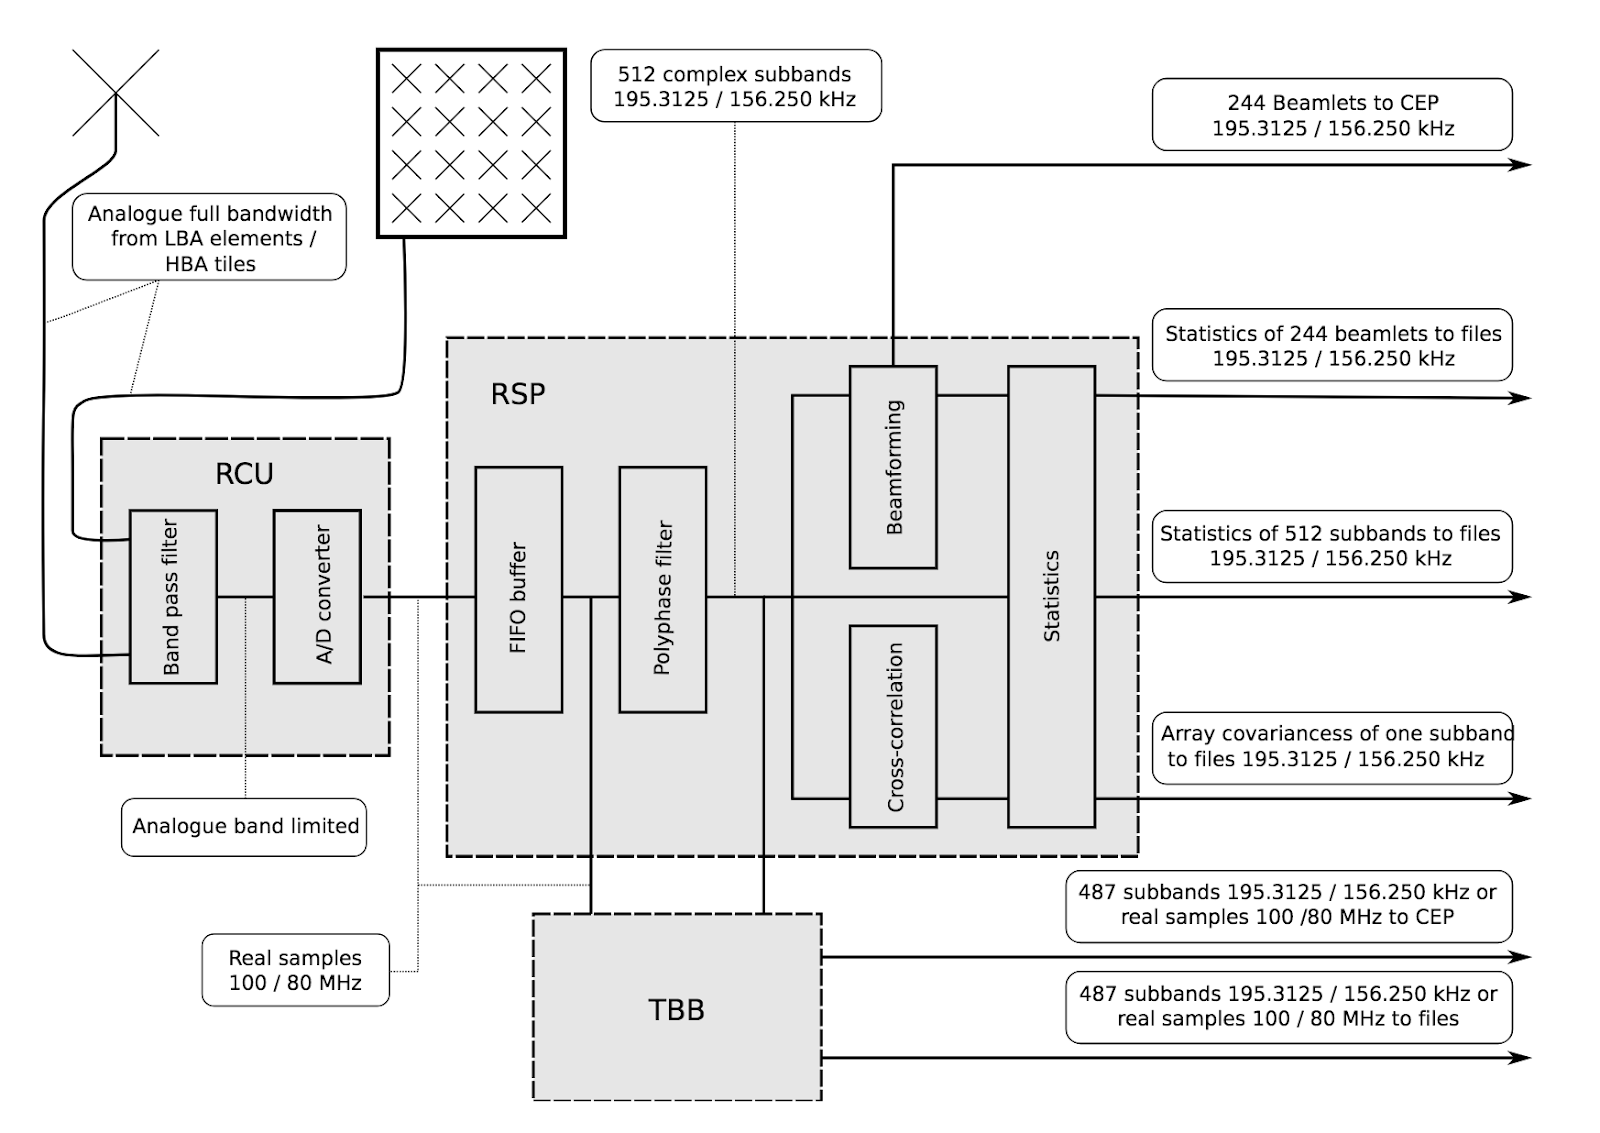
\includegraphics[width=0.75\columnwidth]{Images/Digital_signal_processing.png}
    \caption[Digital signal processing pipeline of an individual LOFAR station.]{Digital signal processing pipeline of an individual LOFAR station. Data is first digitised in the ReCiever Unit (RCU) before being sent to the RSP board. Here data is channelised by a polyphase filter and beamformed before being sent to the CEntral Processor (CEP) in the Netherlands. Also featured is the TBB which stores data in a ring buffer unless it is read out to an external storage system. }
    \label{fig:sig_pipe}
\end{figure}
\subsection{Low Band Antenna}
The LBA consists of two lengths of copper wire which act as a cross dipole antenna, allowing measurements from two linear polarisations. These are connected to a preamplifier placed on top of a PVC pipe. 
Each wire is 1.38 m long which results in a 52MHz resonance peak in power spectra: however, due to the impedance of the amplifier this is increased to 58MHz. A typical LBA power spectrum is shown in Figure \ref{fig:mode3_spec}.
\begin{figure}[t]
    \centering
    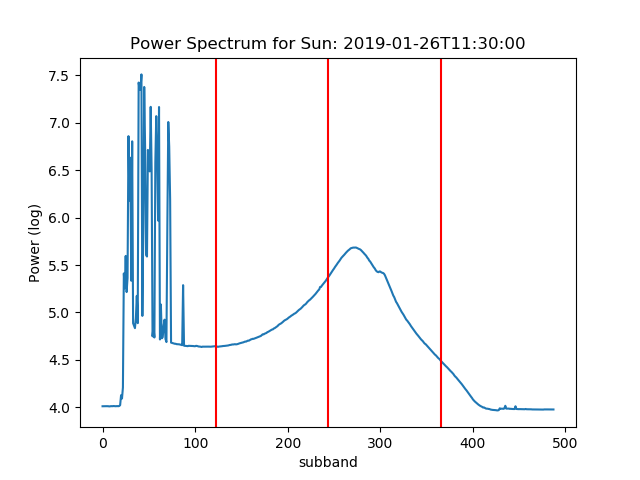
\includegraphics[width=0.75\columnwidth]{Images/Sun_pspec.png}
    \caption[Typical power spectrum for an LBA.]{Typical power spectrum for an LBA. Here the red vertical lines denote the sections of the spectra made from the different RSP lanes (Section \ref{sec:rsp}).}
    \label{fig:mode3_spec}
\end{figure}
The LBA is attached to a steel ground plane made out of concrete reinforcement rods by synthetic rubber straps and polyester rope. The ground plane acts as a reflector for radio waves, increasing the signal received by the antennas.
The simple design of the LBA and the fact that it observes at such low frequencies means that it is sensitive to the entire sky at once. Digital beamforming techniques are used to point an LBA array at a particular location on the sky, the direction of which can be changed in a manner of seconds.
%This pipe is anchored to a metal ground plane made out of steel commonly used in concrete reinforcement by two 1.38m copper wires which act as a cross dipole antenna, thus allowing both X and Y polarisations to be measured. The simple structure of the LBA means that there is a resonance peak at $\sim 58$MHz.
\subsection{High Band Antenna}
The higher frequencies LOFAR can observe at are recorded by the HBAs. The HBA design is drastically different to the simple design of the LBA so that system noise can be reduced. Each HBA is a 5 m $\times$ 5 m tile consisting of 16 bow-tie cross dipole antennae, all aligned in the same direction, supported in an expanded polystyrene structure. The HBA sits on top of a 5 cm $\times$ 5 cm wire mesh ground plane and is encased in two overlapping polypropylene foil layers in order to protect it from the weather. The finer mesh size in the ground plane for a HBA makes it more reflective for the $\sim 10$ cm waves being observed.% The majority of the tile is made out of expanded polystyrene making it lightweight and durable to weather condidtions. 
Each bow-tie antenna in a HBA tile is connected to a front-end which performs preamplification and analogue beamforming. Analogue beamforming is achieved using lengths of copper in a HBA front-end, the same digital beamforming techniques used for LBAs are also used for HBAs.
Each front-end is then connected to a summator where all the signals are summed before being sent for further signal processing in the station container (Section \ref{sec:sig_pipe}). 

\subsection{Remote Station Processing Boards (RSPs)}
\label{sec:rsp}
The RSPs perform all digital signal processing in a LOFAR station. Each LOFAR station consists of 24 RSP boards capable of channelising, beamforming and correlating raw voltage data recorded by either the LBAs or HBAs. A polyphase filter converts recorded data into 1024 complex subband signals which, because the signal is real, is fully described by the positive 512 subbands. These 512 subbands offer $\sim 195$ kHz frequency resolution across the observed band.
In order to perform beamforming, all RSPs are connected together in a ring. Data are passed along this ring and summed in each RSP where a phase correction is also applied in order to ``point" the telescope beam. A maximum of 488 subbands can be used to create beamlets, beams pointed in a particular direction observing in a particular frequency. Data from this process is streamed to an external storage node from 4 points in the ring along what are known as ``lanes" each containing one quarter of the beamlets computed by the RSP boards. 

%Access to the data from RSP boards directly is possible provided there is a sufficient computer back end and network setup capable of writing the data being sent at 3.3Gbps.
\subsection{Transient Buffer Boards (TBBs)}
\label{sec:tbb}
One of the lesser used pieces of LOFAR hardware are the Transient Buffer Boards (TBBs). TBBs are Random Access Memory (RAM) buffers that can temporarily store data at its natively sampled, 5 ns time resolution. Each LOFAR station contains a total of 12 TBBs ranging from 1 GB to 32GB of memory. More recently completed stations such as the Irish LOFAR station (I-LOFAR) have 32GB TBBs while the older Dutch stations usually have less than 16GB.
%A single TBB stores data from 8 different antennas with 2 polaristions each  
A 32 GB TBB can store up to 5 seconds worth of data recorded by a LOFAR station although this can be increased if fewer inputs or polarisations are recorded. TBBs are currently used in analysing cosmic ray showers and lightning storms but have yet to become a mainstream tool for solar physics, despite their potential. 
Recording the radio Sun at 5 ns has never been attempted before and could offer a wealth of never-before-studied phenomena or cast new light onto longstanding questions.

While the next generation telescopes like the Square Kilometre Array (SKA) and the Murchison Widefield Array (MWA) sample at higher rates than 5 ns, no other exisitng radio interferometer stores data at the sampled time resolution. This gives LOFAR the unprecedented ability to capture transient events at their highest temporal resolutions yet.

\section{I-LOFAR: The Irish LOw Frequency ARray}
One of the many benefits to using LOFAR as a radio telescope is that each station can be used independently in Single Station Mode which, in the case of international stations, gives freedom to the host countries to make specific observations that may not be covered in a LOFAR observing cycle. Not only this, but Single Station mode offers the flexibility of the raw complex voltage data before it has passed through any averaging or calibration pipelines that occur during international observing mode. 

The Irish LOFAR station was completed in July of 2017 and is one of the only stations that is used during single station mode to predominantly observe the Sun. A great effort has been made by members of the I-LOFAR consortium, in particular from staff and students Trinity College Dublin and the Dublin Institute for Advanced Studies (DIAS), to maximise the scientific output of I-LOFAR. Collaborating with Griffin Foster of the Breakthrough Foundation and Dr. Brian Coghlan from the School of Computer Science and Statistics has allowed us to develop a real time transient detection computer cluster and software suite to record data from I-LOFAR's RSPs and a second cluster dedicated to the capture of data from the TBBs. %In order to fully understand the challenges posed by recording data in singal station mode, the digital signal processing pipeline for I-LOFAR should be explained. 

This direct access to raw voltage data allows any form of data processing imaginable to be performed. The only limit to this is the computer power and data storage available, two extremely non-trivial problems with LOFAR data. Recording complex raw voltage data from the RSPs requires a 10 Gbps fibre optic link between the LOFAR cabinet and a powerful computer cluster. Due to the unpredictable nature of solar radio bursts, the only way to guarantee they will be recorded is to observe for many hours. Data quickly become terabytes in size which becomes challenging to store and perform any amount of post-analysis.

One disadvantage of using Single Station mode is that the maximum obtainable baseline is $\sim 80$ m corresponding to an angular resolution of $\sim 2.4^{\circ}$ at 90 MHz. Typical angular sizes of active regions on the Sun are $\sim 2^\prime$ thus, any resulting interferometric images are generally too poorly resolved to be of use scientifically. Fortunately, baseline length is not the limiting factor in spectroscopic work, rather sensitivity is. I-LOFAR has a sensitivity of the order of 4 - 200 mJy (1 Jy = $10^{-26} \mbox{ W m}^{-2} \mbox{ Hz}^{-1}$) across its observing band. This is more than sufficient to observe solar radio bursts which have a typical flux of the order of $10^6$ Jy.
Section \ref{sec:sig_pipe} will outline the digital signal processing pipeline for a LOFAR station in Single Station Mode.
%, because the main appeal of LOFAR are its long baseline capabilities, little has been developed for Single Station use which only has

%that you can essentially do whatever you want but in order to record this data in the first place you need a dedicated computer cluster and high speed network connectivity to the LOFAR station. Another disadvantage of using Single Station mode is that, because the main appeal of LOFAR are its long baseline capabilities, little has been developed for Single Station use which only has a maximum baseline of $\sim 300$m.



\subsection{Digital Signal Processing for a Single LOFAR Station}
\label{sec:sig_pipe}
The LOFAR digital signal processing pipeline for a single station is outlined in Figure \ref{fig:sig_pipe}. An analogue signal is received by the High Band Antennas (HBAs) or Low Band Antennas (LBAs). This is sampled at 200 MHz and converted to a digital signal by a 12 bit A/D converter inside the station's Receiver Units (RCUs). Each RCU digitises data for 1 antenna feed (X or Y polarisation) meaning there are $96 \times 2 = 192$ RCUs in total. The digitised data is then sent to the RSP boards. In a standard LOFAR observation while the station is in International LOFAR Telescope (ILT) mode, data from 8 RCUs are channelised into 512 subbands by a polyphase filter bank. This results in raw complex voltage data at 195.3125 kHz frequency resolution and 5.12 $\mu$s temporal resolution which are then phase shifted and added together in order to ``beamform" to a particular location on the sky. The output from each of the 24 RSP boards are added in a ring before being sent along a 10Gbps fibre link to Groningen and passed into the COBALT processing cluster where the data can be further channelised and correlated to produce interferometric or beamformed data products.

The digital signal processing pipeline is much the same in Single Station Mode however, data are averaged to 1 second before being saved as various ``statistics" files. These include subband statistics, which give the power spectrum for each antenna; beamlet statistics, the power in each beamlet formed by the LOFAR station; and crosslet statistics, the correlation coefficients between each antenna which can be used to create all sky images.
Parallel to this, the raw voltage signal with the full 5 ns temporal resolution is stored in the memory of a TBB. A single LOFAR station has 12 TBBs which take 2 RSP boards as inputs each. The buffer will constantly overwrite itself until it is frozen and dumped either by an internal/external trigger signal or sending a dump command manually. In order to store TBB data more permanently, an external storage node is required.



The drastic reduction of 6 orders of magnitude temporal resolution when a station is in Single Station Mode is the main motivation for I-LOFAR to develop its own computer clusters for the storage and processing of data. Alongside this, a dedicated storage node for TBB data will enable I-LOFAR to store its highest time resolution data and allow for a ``DIY radio telescope" style of data processing described in section \ref{sec:tbb_data}

